\chapter{Referencial Teórico}

\section{Princípios e Padrões de Projetos}


Desenvolver software orientado a objetos é um desafio. Criar uma representação
computacional de uma faceta da realidade em que seus constituintes trabalhem de
forma harmoniosa para atingir as necessidades que o software se propõe a
atender requer experiência, conhecimento do domínio do problema e um processo de
análise e projeto. Apesar de existirem várias abordagens para se conceber um
sistema orientado a objetos\cite{evans2004ddd},\cite{gomma11}, um sistema bem
construído apresenta características fundamentais como alta coesão e
baixo acoplamento.

A Coesão é uma característica de um componente de software que se refere ao grau
de relacionamento entres os membros desse componente. No contexto de uma classe,
é levado em consideração as relações entre os métodos e atributos. Classes com
coesão baixa demonstram grande complexidade pois os atributos e métodos que não
se relacionam indicam que a classe tem muitas responsablidades.

O acoplamento descreve as dependências entre componentes. Quanto maior a
quantidade dessas dependências entre classes, mais complexo ela se torna, pois
dificulta  alterações na classe. Além disso, o acoplamento aumenta o risco de
uma classe ser afetada devido à alterações em suas dependências.

Um padrão, dentro do contexto de estudo deste trabalho pode ser definido
como uma técnica efetiva cuja a sua aplicabilidade é aceita e difundida dentro
de uma área de conhecimento com a intenção de atingir um
objetivo\cite{MetskerWake06}. Ao seguir um padrão evita-se o retrabalho de
resolver um problema cuja a solução já existe.

Um padrão de projeto descreve uma solução para algum problema recorrente em um
sistema orientado a objeto \cite{gof}. Essa descrição envolve as motivações para
a utilização daquele padrão, a estrutura de classes e objetos participantes do
padrão e contextualização de sua aplicabilidade. Em desenvolvimento de software,
o catálogo mais difundido de padrões de projetos orientado a objetos é elaborado
por \citeonline{gof}, contendo um total de 23 padrões formalmente documentados
que acumulam experiências bem sucedidas em diversos sistemas. Esses padrões têm
a seguinte classificação:

\begin{description}
\item[Criacionais] Padrões que definem como criar novas instâncias de classes.
\item[Estruturais] Foca na estruturação das classes e objetos.
\item[Comportamentais] Definem como as classes e objetos interagem entre si e
suas responsabilidades.
\end{description}
%argumentação
Analisando a forma como um padrão de projeto é concebido, com uma definição
dos papéis de cada elemento participante e como eles interagem entre si,
pode-se concluir que o uso dos padrões de projeto promove maior coesão, melhor
separação de interesses e baixo acoplamento no sistema. Todas essas
características contribuem para um software de melhor qualidade.


%Melhorar isso

%Linkar com as metricas, mostrar relação metricas e padroes

\section{Métricas de qualidade OO}
\label{sec:metrics}

%A qualidade de software . Segundo \citeonline{pressman}, qualidade de software 
%Qualidade

%Existem aspectos da qualidade de software que podem ser mensurados como
%Alguns aspectos da qualide de software são subjetivos, como por exemplo,
% a facilidade de uso ou manutenabilidade. É possível medir os 

%A classe é a unidade fundamental de um sistema oo

Com o advento de novas técnicas de desenvolvimento de software é necessário
obter informações do impacto dessas inovações nos resultados de um projeto. Com
esse objetivo \citeonline{cksuite} criaram um conjunto de métricas para
medir a qualidade de sistemas desenvolvidos usando o paradigma orientado a
objetos que não se limitasse a uma linguagem de programação, fácil de coletar e
com forte embasamento teórico na ontologia de Bunge que é um modelo usado pra
analisar algumas propriedades estáticas e dinâmicas de um sistema de
informação\cite{WandWeber}. As métricas são:

%Bunge’s ontology has
%considerable appeal for 00 researchers since it deals with the
%meaning and definition of representations of the world, which
%are precisely the goals of the object oriented approach [32]



\begin{description}

\item[Response sets for Class (RFC)] Quantidade de métodos que são executados
quando um objeto recebe uma mensagem, incluindo os métodos de outras classes. É
levado em consideração somente os métodos que são chamados diretamente.

\begin{figure}[!ht]
	\centering
	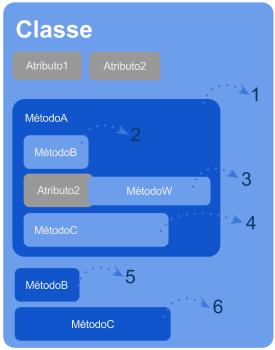
\includegraphics[scale=0.6]{img/pic_rfc.png}
	\caption{Exemplo de avaliação da métrica RFC/Fonte: Próprio Autor}
	\label{fig:pic_rfc}
\end{figure}

Na figura \ref{fig:pic_rfc}, a classe de exemplo tem um total de três métodos
definido nela. A implementação do método ``MetódoA'' chama o método ``MétodoB'',
o método ``MétodoW'' que é de outra classe referenciada pelo atributo
``Atributo2'' e o método ``MétodoC''. Assumindo que os métodos ``MétodoB'' e
``MétodoC'' não contém chamadas a nenhum outro método, o valor da métrica RFC
para a classe ilustrada é de seis métodos.

\item[Coupling Bettwen Objects (CBO)]  Em um sistema orientado a objetos,
diversas classes são implementadas para exercer uma respoonsabilidade, as
instâncias dessa classes interagem entre si para atingir o objetivo do sistema.
Uma classe está acoplada a outra quando o método de um classe invoca o método de
uma variável de instância de outra classe que gera uma dependência entre essas
classes. Quanto mais dependências existirem, mais difícil é reutilizar esses
componentes em outras partes do sistema, além do aumento do risco de efeitos
colaterais que ocorrerem ao modificar uma classe altamente acoplada. O valor da
métrica CBO para uma classe é o número de outras classes que a classe analisada
depende.

\begin{figure}[!ht]
	\centering
	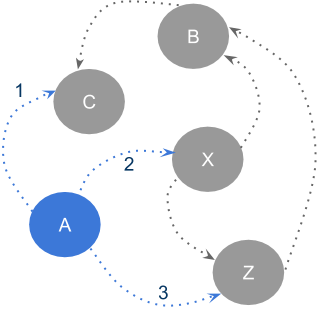
\includegraphics[scale=0.8]{img/pic_cbo.png}
	\caption{Exemplo de avaliação da métrica CBO/Fonte: Próprio Autor}
	\label{fig:pic_cbo}
\end{figure}

A figura \ref{fig:pic_cbo} ilustra um exemplo de acoplamento entre objetos. Um
classe chamada ``A'' depende das classes ``C'', ``X'' e ``Z''. O
valor de CBO para a classe ``A" é a somas de todas as suas
dependências, neste caso totalizando três dependências.


\item[Lack of Cohesion in Methods (LCOM)] Usado para avaliar a coesão de uma
classe por meio dos relacionamentos entre seus atributos e métodos.
O valor dessa métrica é fornecido por meio da quantidade de métodos que não tem
nenhum atributo em comum, menos a quantidade de métodos que tem atributos em
comum.

\begin{figure}[!h]
	\centering
	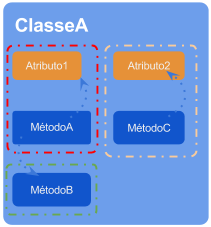
\includegraphics[scale=0.8]{img/pic_lcom_ex1.png}
	\caption{Exemplo  de avaliação da métrica LCOM/Fonte: Próprio Autor}
	\label{fig:pic_lcom_ex1}
\end{figure}

No exemplo da figura \ref{fig:pic_lcom_ex1} a classe ilustrada tem três métodos
implementados e cada método tem um conjunto de atributos que cada um utiliza.
O método ``MétodoA'' utiliza o atributo ``Atributo1'' formando o cunjunto Ma =
\{Atributo1\}, o método ``MétodoB'' não utiliza nenhum atributo formando um
conjunto vazio Mb = \{\}, e o método ``MetodoC'' referencia o atributo
``Atributo2'' formando o conjunto Mc = \{Atributo2\}. É necessário descobrir a
interseção de cada um desses grupos para saber quantos grupos tem atributos em
comum. A seguir é mostrado o resultado dessa avaliação:

\[
Ma \cap Mb = \{ \},
Ma \cap Mc = \{ \},
Mc \cap Mb = \{ \}
\]

Com esses resultados em mãos pode-se calcular o valor de lcom para a classe
exemplos. O total de conjuntos resultates vazios é três  e não foi identificado
nenhum conjunto com algum atributo que seja compartilhado entre os métodos.
Portanto o LCOM para para a classe ``ClasseA'' é, três conjuntos vazios, menos
zero conjuntos não vazios, que é igual a, LCOM três.

\begin{figure}[!h]
	\centering
	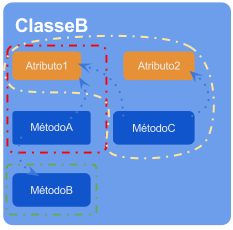
\includegraphics[scale=0.8]{img/pic_lcom_ex2.png}
	\caption{Exemplo  de avaliação da métrica LCOM/Fonte: Próprio Autor}
	\label{fig:pic_lcom_ex2}
\end{figure}

Outro exemplo é mostrado na figura \ref{fig:pic_lcom_ex2} . Aplicando a mesma
nomenclatura do exemplo anterior da figura \ref{fig:pic_lcom_ex1} teremos a
seguinte analise para calcular o valor de LCOM para a classe ``ClasseB'': Dado,
Ma = \{ Atributo1\}; Mb = \{\}; Mc = \{Atributo1, Atributo2\}. 

\[
Ma \cap Mb = \{ \},
Ma \cap Mc = \{ Atributo1 \},
Mc \cap Mb = \{ \}
\]

Totalizando dois conjuntos vazios e um conjunto não vazio. Portanto o valor da
métrica LCOM para a classe ``ClasseB'' é de um conjunto. Podemos concluir que a
classe ``ClasseB'' é mais coesa que  a classe ``ClasseA''.


\item[Depth Inheritance Tree (DIT)] Nível de uma classe na
hierarquia de herança. Reflete o número máximo de nós  dentro da árvore
de classes até a raiz, o que aumenta a complexidade conforme a quantidade de
elementos envolvidos se eleva, diminuindo a previsibilidade do comportamento da
classe com vários métodos e atributos sendo herdados, principalmente com o uso
de sobrecarga de métodos. No exemplo da figura \ref{fig:pic_dit} a classe
``ClasseZ'' tem um relacionamento de herança com a classe ``ClasseT'' que se
relaciona também por meio de herança com a classe ``Raiz''. A distância entre a
classe ``ClasseZ'' até a classe ``Raiz'' na hierarquia é de dois nós. Portanto o
valor da métrica DIT para a classe ``ClasseZ'' é dois.

\begin{figure}[!ht]
	\centering
	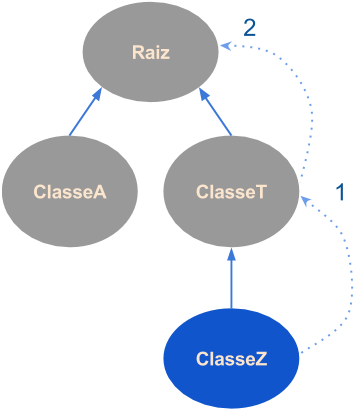
\includegraphics[scale=0.6]{img/pic_dit.png}
	\caption{Exemplo de avaliação da métrica DIT/Fonte: Próprio Autor}
	\label{fig:pic_dit}
\end{figure}

\item[Number of Children (NOC)] Número de subclasses imediatas de uma
classe analisada. Essa medida é um indicativo de mau uso de herança conforme seu
valor aumenta e mostra o impacto que uma classe pode ter no sistema requerendo maior
atenção e testes.

\begin{figure}[!ht]
	\centering
	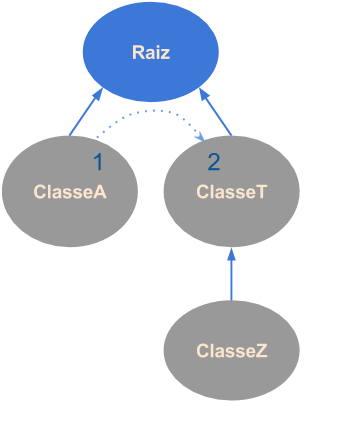
\includegraphics[scale=0.6]{img/pic_noc.png}
	\caption{Exemplo de avaliação da métrica NOC/Fonte: Próprio Autor}
	\label{fig:pic_noc}
\end{figure}

Na figura \ref{fig:pic_noc} a classe ``ClasseA'' e a classe ``ClasseT'' são as
únicas classes que tem uma relação de herança direta com a classe ``Raiz'',
portanto o valor da métrica NOC para a classe ``Raiz'' é  dois.

 

\item[Wheighted Methods per Classe (WMC)] Serve para expressar o nível de
complexidade de uma classe com base na soma da complexidade dos métodos que ela
possui. Isso afeta o esforço de manutenção da classe, além de impactar nas
classes filhas que herdarão esses métodos. Também é um indicativo de que a
classe tem métodos específicos dificultando o seu reuso. A unidade de
complexidade definida por \citeonline{cksuite} é o próprio método e não
considera outros fatores como número de linhas, número de parâmetros ou
quantidade de estruturas de decisão. A figura~\ref{fig:pic_wmc} ilustra como a
métrica WMC é avaliada em uma classe.

\begin{figure}[!ht]
	\centering
	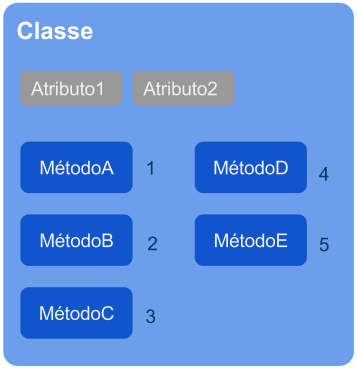
\includegraphics[scale=0.6]{img/pic_wmc.png}
	\caption{Exemplo de avaliação da métrica WMC/Fonte: Próprio Autor}
	\label{fig:pic_wmc}
\end{figure}

No exemplo da figura~\ref{fig:pic_wmc}, a classe reprensentada tem um total de
cinco métodos implementados. Seguindo estritamente o que \citeonline{cksuite}
definem para a métrica, o valor da métrica WMC para a classe é cinco métodos.


\end{description}

Todas essas métricas tem uma relação inerente com a coesão e acoplamento dos
objetos, sendo uma forma confiável para a análise da qualidade em sistemas
orientados a objetos. Os aplicativos desenvolvidos para a plataforma android são
escritos usando a linguagem de programação Java que emprega esse paradigma de
desenvolvimento, o que justifica o uso das métricas de \citeonline{cksuite} para
validação dos projetos orientados a objetos.

\section{Model View Controller}

O padrão \textit{Model View Controller} surgiu como uma solução genérica para
que usuários de um sistema de planejamento manipulem dados complexos
\citeonline{Reenskaug:1979}. Posteriormente, \citeonline{krasnerPope1988}
implementam um framework MVC para o ambiente gráfico da linguagem de programação
Smalltalk-80 como uma forma de promover a reusabilidade e plugabilidade dos
componentes de um sistema.

Segundo \citeonline{Reenskaug:1979} o principal objetivo do MVC
``\ldots é representar o modelo mental do usuário de um espaço de informações
relevantes e permitir que o usuário inspecione e altere estas
informações.''(tradução livre).
Esse modelo mental é como o usuário percebe o dominio do problema que está inserido no qual executará suas atividades sobre dados de seu interesse. Para que o usuário de um sistema de
informação possa interagir com a representação computacional  de seu modelo
mental três componentes são definidos:

Model - É o componente constituído de uma composição de classes que implementam
as regras de negócio referentes as funcionalidades que o programa provê,
representa o  conhecimento que o usuário tem e como manipulá-lo. Atende
mensagens da view requisitando seu estado e mensagens do controller para mudar
seu estado,

View - Representação específica de um model na interface com o usuário, é 
responsável por toda a manipulação visual, recuperando um estado do model e
exibindo os dados, podendo ser composta por sub-views e ser parte de views mais
complexas.

Controller - Interpreta as ações do usuário provenientes de um dispositivo de
entrada(Teclado, Mouse) alterando estado da view ou do model.




\citeonline{krasnerPope1988} descrevem a estrutura do MVC onde a view tem seu
controller exclusivo mantendo uma dependência cíclica entre ambos. Tanto a View
quanto o Controller tem referências diretas para o model por meio de atributos
de classe, porém, o model não deve conhecer seus respectivos pares de
View-Controller para promover maior reuso de código e encapsulamento do model.
As alterações do estado do model são feitas na maioria das vezes pelo controller, e
o model é responsável por notificar todas as views que o representa para que
se atualizem refletindo o novo estado. No caso de um model ser usado por vários
pares de View-Controller as mensagens de notificação de um novo estado do model
podem ser parametrizadas assim cada view pode verificar se a alteração é de seu
interesse. 

Segundo \citeonline{Fowler:2002:PEA} ``\ldots esta separação da
apresentação e modelo é uma das mais fundamentais heurísticas de bom projeto
de software''(tradução livre).
O controller poderia ser o responsável por publicar as alterações no estado do
model devido sua relação direta com o mesmo, mas em casos onde o model é
alterado por outro componente que não é um dos controladores que os utilizam, é
necessário que o model conheça as views que devem ser notificados do novo
estado. Para que essas alterações de estado sejam propagadas a view e o
controller são registrados como dependentes de seu model. O padrão é descrito
levando em consideração as aplicações desenvolvidas em Smalltalk usando
características espefíficas dessa linguagem de programação que da suporte à
implementação dos três componentes como por exemplo o gerenciamento dos objetos
que são dependentes do model definido na classe Object que o model deve
extender. A Figura \ref{mvc} esclarece a interação entre os componentes.



\begin{figure}[htb]
	\caption{\label{mvc}Representação dos componentes do MVC}
	\begin{center}
		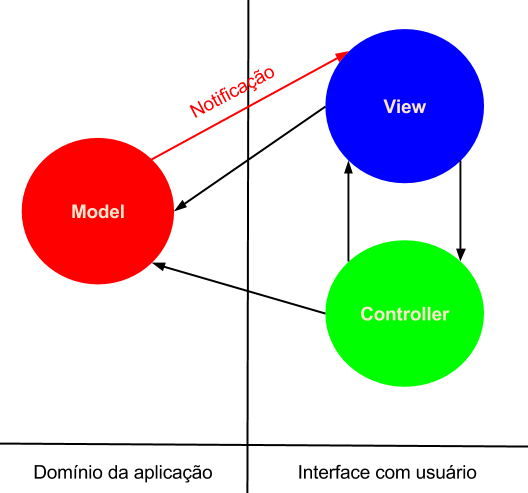
\includegraphics[scale=0.5]{img/mvc.png}
	\end{center}
	\legend{Fonte: Próprio Autor}
\end{figure}

\citeonline{gof} cita \citeonline{krasnerPope1988} fazendo uma análise dos
objetos que compõem o MVC relacionando-os com outros padrões de projeto
descritos em seu catálogo.
O desacoplamento entre a View e o Model, somado à propagação das mudanças de
estado no model para a View e o Controller podem ser
descritos como uma implementação do padrão Observer. Segundo \cite{gof} o padrão
Observer ``\ldots Define uma dependência de 1-N entre objetos para quando um
objeto mudar de estado, todos os seus dependentes são notificados e atualizados
automaticamente''(tradução livre). \citeonline{krasnerPope1988} descrevem essa
estrutura com o conceito de Dependents onde a View e o Controller são
registrados como dependentes do model. O padrão Observer é composto por uma
estrutura em que um objeto precisa publicar mudanças em seu estado, detém a
referência para os objetos a serem notificados. A organização das classes de
acordo com o que o padrão descreve permite que várias Views possam se atualizar
dada uma modificação no Model.

A View é composta por vários objetos com a responsabilidade em comum de
representar parte ou todo o estado do Model. Este é um exemplo do padrão de
projeto Composite. Segundo \citeonline{gof} o padrão Composite ``\ldots
Integra objetos em uma estrutura de árvore para representar uma hierárquia
parte-todo, deixando clientes tratar objetos individuais e composições de
objetos uniformemente''(tradução livre).Uma view pode ser constituída por
sub-views para compor Views complexas. No Composite  um conjunto de componentes
visuais podem ser tratadas de forma encapsulada onde cada um implementa a
mesma abstração. 

Segundo \citeonline{gof} o padrão de projeto Strategy ``\ldots define uma
família de algorítmos, encapsula cada um, e torna-os substituíveis entre si
permitindo que variem independentemente dos clientes que o usam''(tradução
livre). O padrão Strategy define uma abstração cuja as implementações podem ser
trocadas de acordo com algum critério. Esse conceito pode ser aplicado ao
Controller que encapsula o algoritmo que vai alterar a View e o Model,
permitindo sua substituíção, por exemplo, por uma outra implementação que deixa
de responder às interações com o usuário.

Segundo \citeonline{krasnerPope1988} o Model ``\ldots pode ser simples como
um valor numério inteiro (como o modelo de um contador) ou um valor literal
(como o modelo de um editor de texto), ou pode ser um objeto complexo''(tradução
livre). O Model pode ser implementado usando o padrão Facade para simplificar
as interações entre o Controller e o Model. O padrão Facade provê
uma abstração mais simples e unificada de várias interfaces de um
subsistema\cite{gof}. Esta forma de interpretar o Model pode ser aplicada
dependendo da complexidade do domínio que ele representa.

\section{Model View Presenter}

O MVP é um modelo de programação para implementação de interfaces com o usuário
desenvolvido como um framework para C++ e Java, criado por uma subsidiária da
IBM chamada Taligent,Inc. Este padrão é baseado no MVC e descreve vários
componentes que tem as responsabilidades de como gerenciar os dados da aplicação
e como o usuário interage com esses dados, tendo como objetivo promover o
encapsulamento do Model , reuso de lógica de negócio e o polimorfismo da View.
São Eles:

\begin{description}
  \item[Model] Tem as mesmas responsabilidades que o Model definido pelo MVC.
  \item[Selections] - Abstração para selecionar um subconjunto dos dados
  existentes no model.
  \item [Commands] Representa as operações a serem executadas sobre uma
  Selection do Model.
  \item [View] Responsável por exibir o model assim como no MVC.
  \item [Interactor] Mapeia os interações do usuário na view como eventos do
  mouse.
  \item [Presenter] O papel do presenter é interpretar o eventos iniciados pelo
  usuário executando a lógica de negócio correspondente implementada em um
  command para manipular o model \cite{Potel96mvp}.
\end{description}


Os conceitos do MVP são descritos em \citeonline{Potel96mvp} de forma genérica
permitindo interpretações para uma implementação efetiva.
\citeonline{twisttriad:2000} descrevem a implementação de um framework para
Dolphin Smalltalk\footnote{Implementação da Linguagem de programação Smalltalk - 
\url{http://www.object-arts.com}} adotando os conceitos do MVP onde salienta que
a maioria dos sistemas operacionais com ambiente gráfico fornece um conjunto de
componentes (Widgets) nos quais estão contidas as responsabilidades do
Controller, de acordo com a descrição do padrão MVC. A maior parte do
comportamento com o usuário é implementada no Presenter que está
diretamente associado à View.

Ainda acerca das responsabilidades do Presenter, \citeonline{fowler:ui} descreve
o que é chamado de Passive View, onde toda a lógica do comportamento da view é
implementado no presenter deixando a view enxuta com o intuito de isolar ao
máximo a API gráfica do resto da aplicação. Dessa forma o model não se comunica
com a view por meio do padrão Observer, sendo que a view séra atualizada
pelo presenter como pode ser observado na Figura~\ref{fig:mvp_passive_view}.

\begin{figure}[ht]
	\centering
	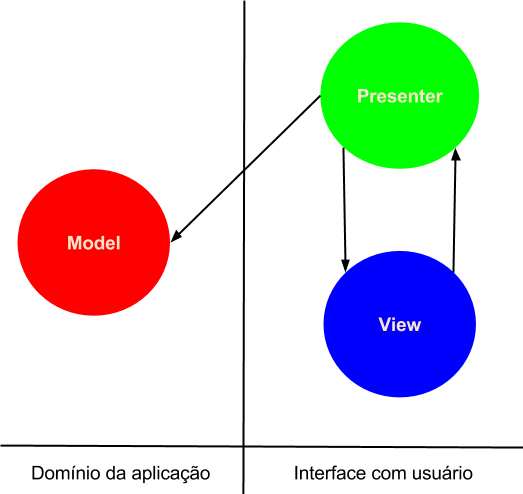
\includegraphics[scale=0.5]{img/passive_view.png}
	\caption{Passive View/Fonte: Próprio autor}
	\label{fig:mvp_passive_view}
\end{figure}

Outra variação do MVP descrita por \citeonline{fowler:sp} é o Supevising
Controller. Nesta abordagem o Model utiliza algum mecanismo de notificação, por
exemplo o padrão Observer, para atualizar a View. Este comportamente é parecido
com o do padrão MVC como pode pode ser observado na
figura~\ref{fig:sup_controller}.

\begin{figure}[ht]
	\centering
	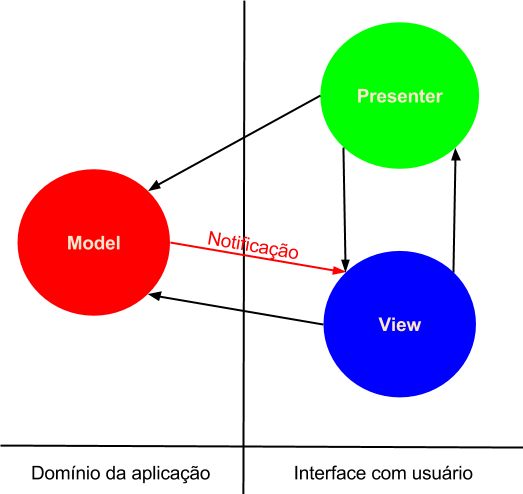
\includegraphics[scale=0.5]{img/supervising_controller.png}
	\caption{Supervising Controller/Fonte: Próprio autor}
	\label{fig:sup_controller}
\end{figure}


MVP se adequa melhor as API's gráficas existentes e define de forma mais clara
os componentes necessários para desenvolver uma aplicação, sendo o ponto de maior
discussão reside em quais os limites das responsabilidades no que tange a
mediação do Model e a View por parte do Presenter.



\section{Framework Android}
 

O android é uma plataforma baseado no linux mantido pela Google para
ser embarcado em dispositivos podendo ser aplicado em carros, televisão, placas
controladoras mas seu destaque é a utilização em smartphones e
tablets, que é o foco deste trabalho. A plataforma é constituída por API's e
frameworks tendo em sua base o sistema operacional e seus drivers seguido da
máquina virtual que executa os aplicativos android e bibliotecas auxiliares e
aplicativos básicos como é demonstrado na figura \ref{android_stack}.

\begin{figure}[h]
	\centering
	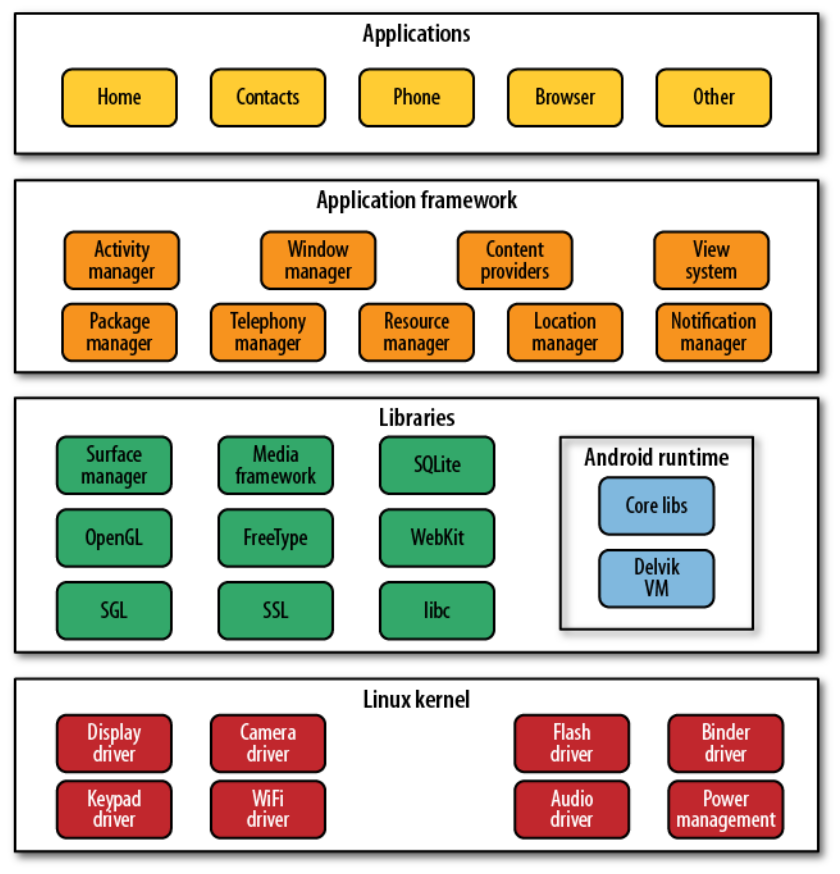
\includegraphics[scale=0.5]{img/android_stack.png}
	\caption{Android Stack/Fonte: Learning Android}
	\label{android_stack}
\end{figure}

Para desenvolvimento é usada a API disponível no SDK que define
os blocos de construção de um aplicativo, a saber:

\begin{description}
  \item[Activity] Representa uma atividade que o usuário executa no aplicativo
  em um determinado momento. É um agregador de componentes visuais e responde à
  interações do usuário.
  \item[Fragment] Representa uma parte de interface com o usuário em uma
  Activity.
  \item[Service] Responsável por executar uma operação sem interface gráfica
  indicado para processamentos longos como por exemplo a execução de uma música
  ou download de de arquivos.
  \item[Broadcast Receiver] Implementação do padrão publish/subscribe 
  \item[Content Provider] Usado para expor dados de uma aplicativo para outros
  aplicativos. Os dados podem ser provenientes de qualquer forma de
  armazenamento como um arquivo ou banco de dados.
  \item[ApplicationContext] Representa a aplicação em execução provendo acesso
  a recursos.
  \item[AsyncTask] Usado para facilitar o uso de Threads evitando o uso
  da linha de execução principal do aplicativo que é respoonsável por tratar a
  interações com o usuário.
\end{description}

Com base nos componentes de framework e literatura revisada é possível fazer
uma análise dos mesmos e projetar uma camada de apresentação utilizando o padrão
MVP para ser usada como referência de implementação a ser aplicada.